\documentclass[aspectratio=169,11pt]{beamer}

% --- CleanEasy theme (installed at ~/beamer) ---
\usetheme{CleanEasy}

\usepackage{booktabs}
\usepackage{amsmath}
\usepackage{xspace}
\usepackage{xeCJK}
\setCJKmainfont{Noto Sans CJK TC}
\setCJKsansfont{Noto Sans CJK TC}
\usepackage{tikz}
\usetikzlibrary{positioning,arrows.meta,fit,backgrounds,shadows}

\graphicspath{{figs/}}

\newcommand{\gpgomea}{GP-GOMEA\xspace}
\newcommand{\exactgpu}{\texttt{gpu\_exact\_gom}}
\newcommand{\batchgpu}{\texttt{gpu\_batch\_gom}}
\newcommand{\cpuoriginal}{\texttt{cpu\_original}}
\newcommand{\aq}{\operatorname{AQ}}

\title[GPU GP-GOMEA]{Accelerating GP-GOMEA for Symbolic Regression}
\subtitle{Exact and Batched GPU Fitness Evaluation}
\author[Team 31]{黃紹祈 (r14921035) \and 賴柏瑄 (r13921098) \and 傅皓群 (r14943177)}
\institute{Team 31}
\date{\today}

\begin{document}

\begin{frame}[plain]
  \titlepage
\end{frame}

%==================================================================
\section{Motivation}

\begin{frame}{The bottleneck in GP-GOMEA}
  \begin{itemize}
    \item \gpgomea finds \textbf{compact} symbolic-regression models via linkage learning + Gene-pool Optimal Mixing (GOM).
    \item GOM evaluates \textbf{many small, sequentially dependent} candidate moves per generation.
    \item Each move accepts/rejects \textbf{immediately} — the next candidate depends on the last.
  \end{itemize}
  \vfill
  \begin{block}{The tension}
    Fitness is data-parallel $\Rightarrow$ GPU-friendly.\\
    One small candidate per launch $\Rightarrow$ launch overhead can exceed CPU cost.
  \end{block}
\end{frame}

\begin{frame}{Engineering and algorithmic questions are inseparable}
  \begin{itemize}
    \item How can GOM expose \textbf{enough parallel work} for a GPU?
    \item What \textbf{search distortion} appears when candidate decisions are \textbf{batched}?
  \end{itemize}
  \vfill
  \begin{exampleblock}{Contributions}
    \begin{enumerate}
      \item CUDA fitness path: trees $\to$ postfix programs, one program per CUDA block.
      \item \textbf{Control-flow exact} vs.\ \textbf{delayed-commit batched} backends.
      \item Orchestration optimizations (CUDA Graphs, pinned buffers, fp32, caches).
      \item Acceleration \emph{and} fitness-distortion measurement.
    \end{enumerate}
  \end{exampleblock}
\end{frame}

%==================================================================
\section{Design}

\begin{frame}{Three backends, one source tree}
  \centering
  \small
  \begin{tabular}{lp{2.6cm}p{3.2cm}p{2.0cm}}
    \toprule
    Backend & Candidate grouping & Accepted-move visibility & Arithmetic \\
    \midrule
    \cpuoriginal & one candidate & immediate & host fp32 \\
    \exactgpu & one candidate & immediate & device fp32 \\
    \batchgpu & multiple candidates & after batch decisions & device fp32 \\
    \bottomrule
  \end{tabular}
  \vfill
  \begin{itemize}
    \item \exactgpu: preserves GOM ordering; not bitwise-identical (reduction order).
    \item \batchgpu: delays donor visibility $\Rightarrow$ \textbf{approximate search variant}.
  \end{itemize}
\end{frame}

\begin{frame}{GPU fitness path}
  \centering
  \begin{tikzpicture}[
    node distance=7mm and 10mm,
    box/.style={draw, rounded corners=2pt, align=center, minimum height=10mm,
                minimum width=23mm, font=\scriptsize\bfseries, thick,
                drop shadow={shadow xshift=0.6pt, shadow yshift=-0.6pt, opacity=0.25}},
    host/.style={box, draw=MediumBlue, top color=MutedBlue, bottom color=MediumBlue!30, text=DarkBlue},
    gpu/.style={box, draw=MediumGreen, top color=MutedGreen, bottom color=MediumGreen!35, text=MediumGreen!50!black},
    dec/.style={box, draw=MediumRed, top color=MutedRed, bottom color=MediumRed!30, text=MediumRed!55!black},
    arrow/.style={-{Stealth[length=2.4mm]}, line width=0.7mm},
    lbl/.style={font=\tiny\itshape}]

    % stage boxes
    \node[host] (tree) {Host tree\\+ FOS move};
    \node[host, right=of tree] (tok) {Postfix\\token program};
    \node[host, right=of tok] (buf) {Pinned host\\buffer};
    \node[gpu,  right=of buf] (ker) {CUDA stack\\interpreter};
    \node[gpu,  below=of ker] (smp) {Threads $=$\\samples};
    \node[dec,  below=of tree] (dec) {Accept /\\reject move};

    % phase background bands
    \begin{scope}[on background layer]
      \node[rounded corners=4pt, fill=MediumBlue!8, draw=MediumBlue!40, dashed,
            fit=(tree)(buf), inner sep=4mm, label={[lbl,text=MediumBlue]above:HOST}] {};
      \node[rounded corners=4pt, fill=MediumGreen!10, draw=MediumGreen!50, dashed,
            fit=(ker)(smp), inner sep=4mm, label={[lbl,text=MediumGreen!50!black]above:GPU}] {};
    \end{scope}

    % arrows
    \draw[arrow, MediumBlue]  (tree)--(tok);
    \draw[arrow, MediumBlue]  (tok)--(buf);
    \draw[arrow, MediumGreen] (buf)--(ker);
    \draw[arrow, MediumGreen] (ker)--(smp);
    \draw[arrow, MediumRed]   (smp)--(dec);
    \draw[arrow, MediumRed, dashed] (dec)--(tree)
      node[lbl, midway, left=1pt, text=MediumRed!60!black]{loop};
  \end{tikzpicture}
  \vfill
  \footnotesize
  One program $\to$ one block; warp lanes process different samples.\\
  Structural tree divergence kept \emph{across} blocks, out of the warp.
\end{frame}

\begin{frame}{Postfix representation \& optimizations}
  \begin{columns}[T]
    \begin{column}{0.5\textwidth}
      \textbf{Representation}
      \begin{itemize}\small
        \item No \texttt{Node*}/\texttt{Op*} on device.
        \item Token: opcode, feature idx, constant.
        \item Fixed-stride padded batch buffer.
        \item Function set $\{+,-,\times,\aq\}$,
          \[\aq(a,b)=\tfrac{a}{\sqrt{1+b^2}}\]
      \end{itemize}
    \end{column}
    \begin{column}{0.5\textwidth}
      \textbf{Overhead reduction}
      \begin{itemize}\small
        \item Single-precision device data.
        \item Pinned, reused host buffers.
        \item \textbf{CUDA Graph replay} (exact).
        \item Capacity-managed device buffers.
        \item Cached subtree / serialization vectors.
      \end{itemize}
    \end{column}
  \end{columns}
\end{frame}

%==================================================================
\section{Results}

\begin{frame}{RQ1 — Exact GPU crossover}
  \begin{columns}[c]
    \begin{column}{0.55\textwidth}
      \centering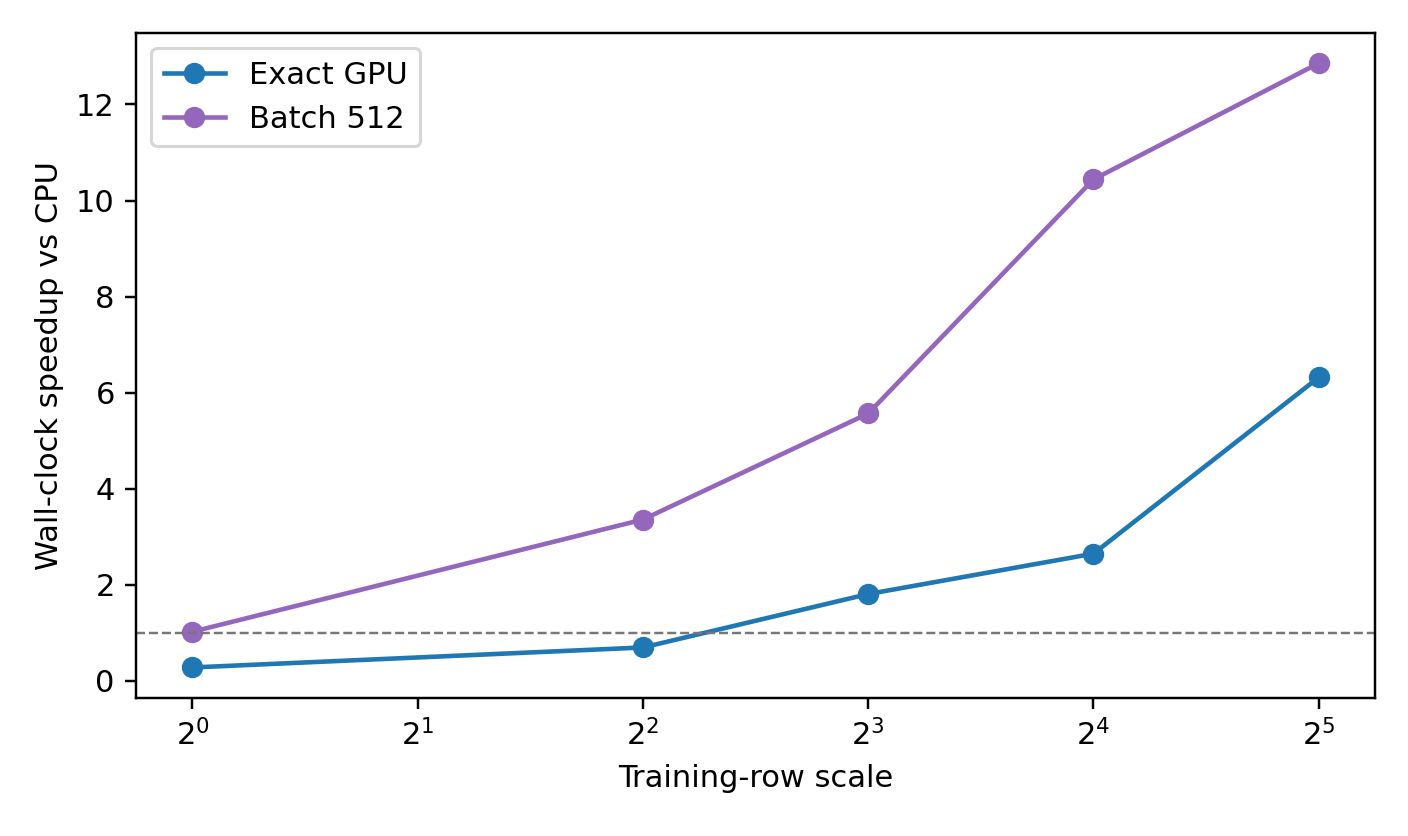
\includegraphics[width=\linewidth]{rowscale_crossover}
    \end{column}
    \begin{column}{0.45\textwidth}
      \begin{itemize}\small
        \item Median \textbf{1.97$\times$} vs CPU (95\% CI 1.76--2.14).
        \item Faster than CPU in \textbf{77\%} of runs; max \textbf{10.20$\times$}.
        \item Rises to \textbf{3.61$\times$} at the largest row scale.
      \end{itemize}
      \begin{block}{Mechanism}
        \small Exact GPU pays off once each candidate has enough sample work to amortize launch.
      \end{block}
    \end{column}
  \end{columns}
\end{frame}

\begin{frame}{RQ1/RQ2 — Speedup vs scale}
  \begin{columns}[c]
    \begin{column}{0.5\textwidth}
      \centering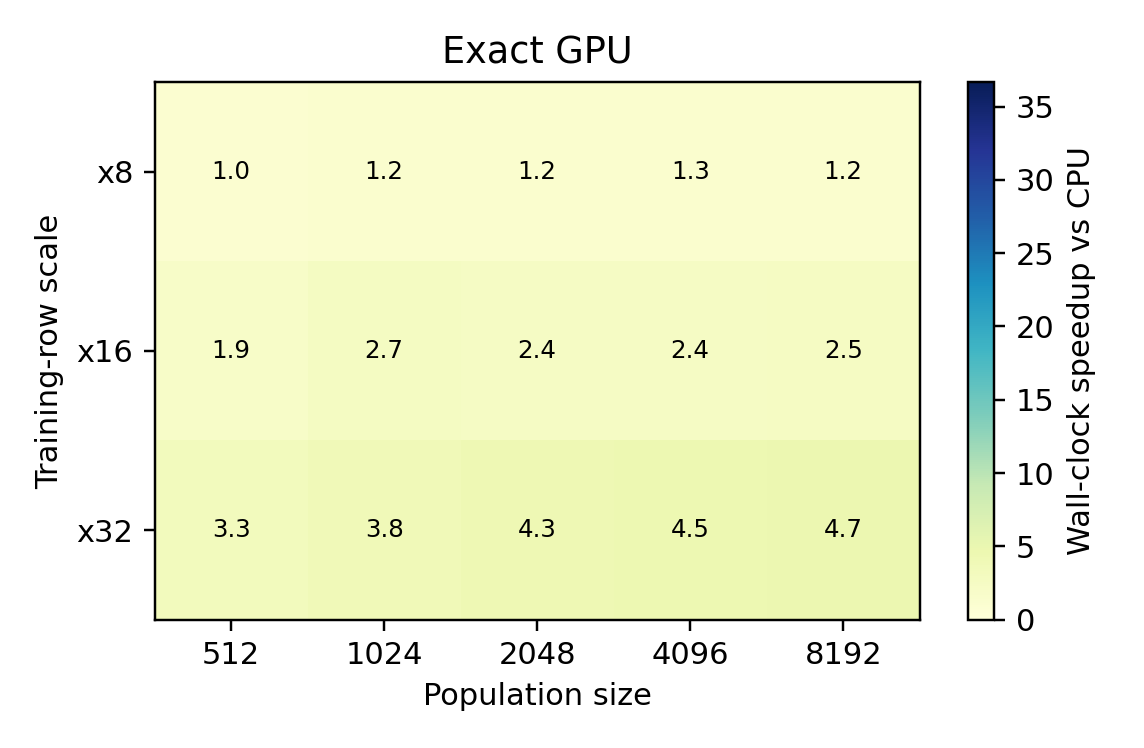
\includegraphics[width=\linewidth]{exact_heatmap}\\
      {\footnotesize Exact GPU}
    \end{column}
    \begin{column}{0.5\textwidth}
      \centering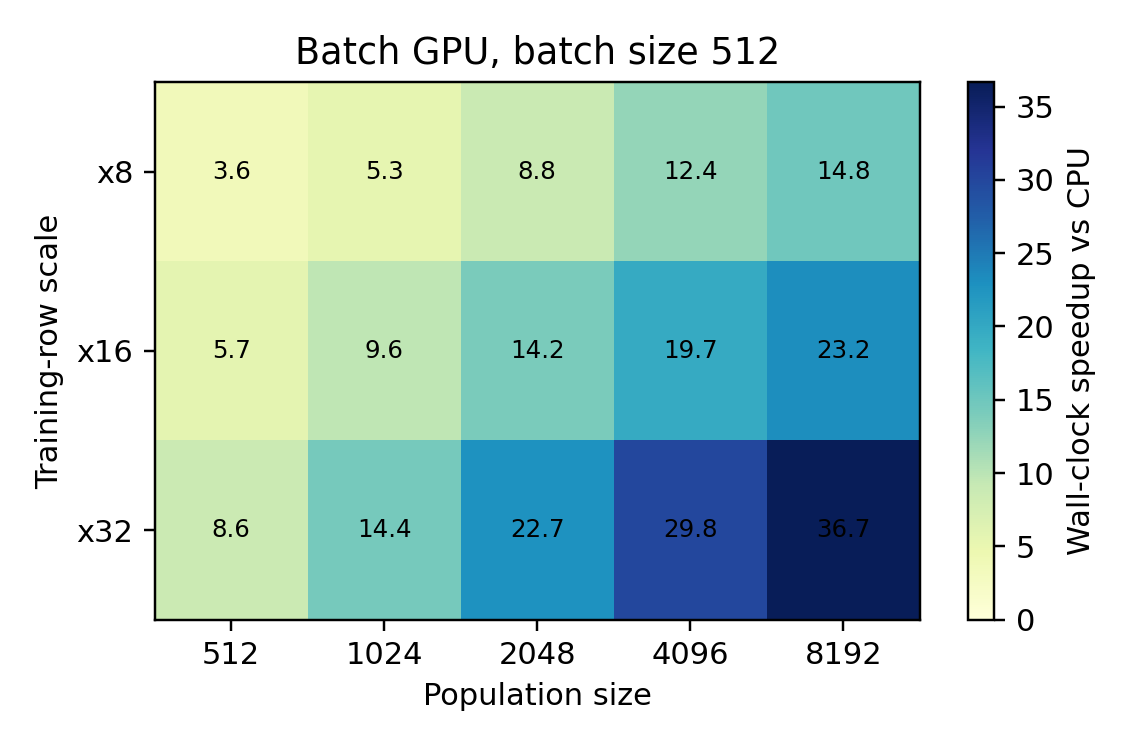
\includegraphics[width=\linewidth]{batch_heatmap}\\
      {\footnotesize Batch GPU (size 512)}
    \end{column}
  \end{columns}
  \vfill
  \centering\footnotesize
  Batching exposes program-level parallelism $\Rightarrow$ best median \textbf{12.27$\times$}, max \textbf{63.24$\times$}.
\end{frame}

\begin{frame}{RQ3 — Batching changes the search}
  \begin{columns}[c]
    \begin{column}{0.55\textwidth}
      \centering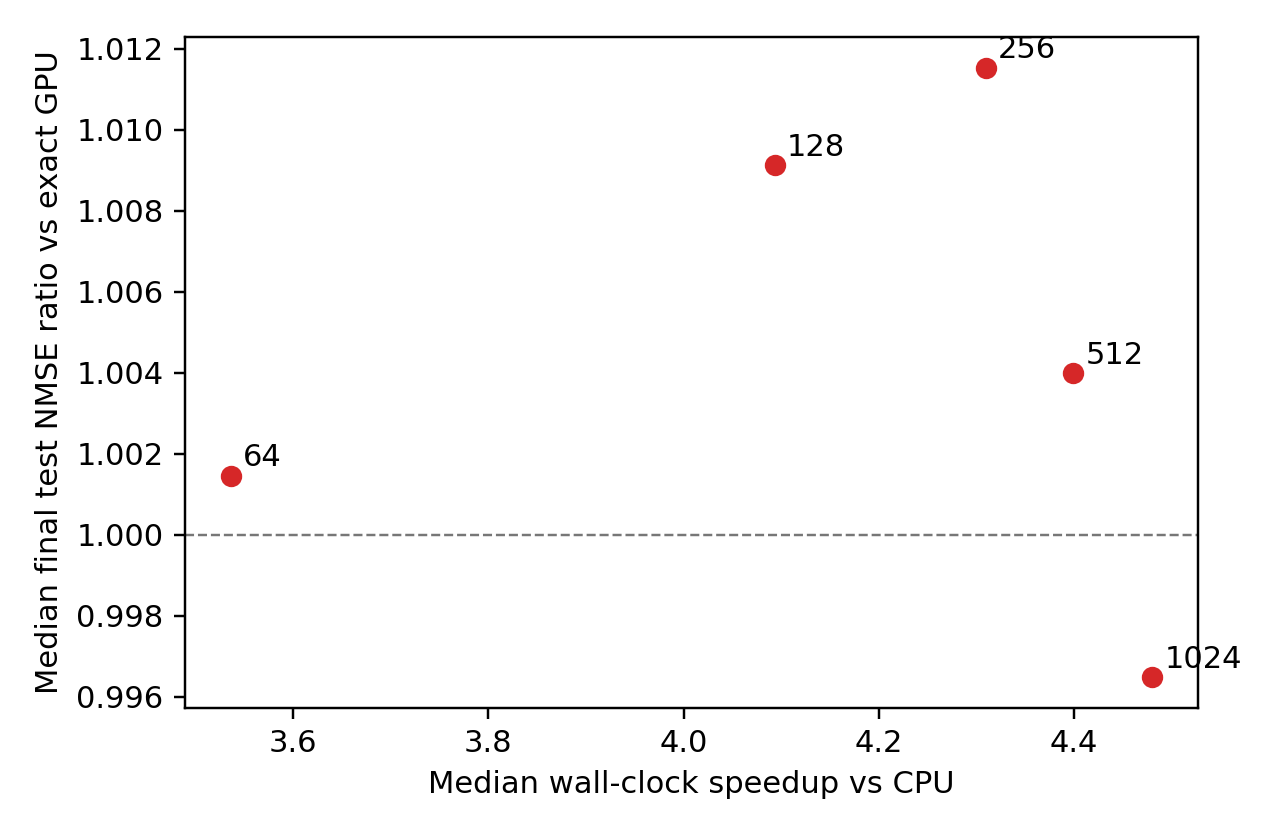
\includegraphics[width=\linewidth]{quality_speed}
    \end{column}
    \begin{column}{0.45\textwidth}
      \begin{itemize}\small
        \item \exactgpu $\approx$ CPU quality (median ratio \textbf{1.000}).
        \item Distortion is \textbf{non-monotonic} in batch size.
        \item More throughput $\neq$ lower error at fixed generations.
      \end{itemize}
      \begin{alertblock}{Takeaway}
        \small Treat \batchgpu\ as a separate \emph{approximate} \gpgomea variant — tune batch size as a hyperparameter.
      \end{alertblock}
    \end{column}
  \end{columns}
\end{frame}

\begin{frame}{RQ3 — Fitness evolution (100 generations)}
  \centering
  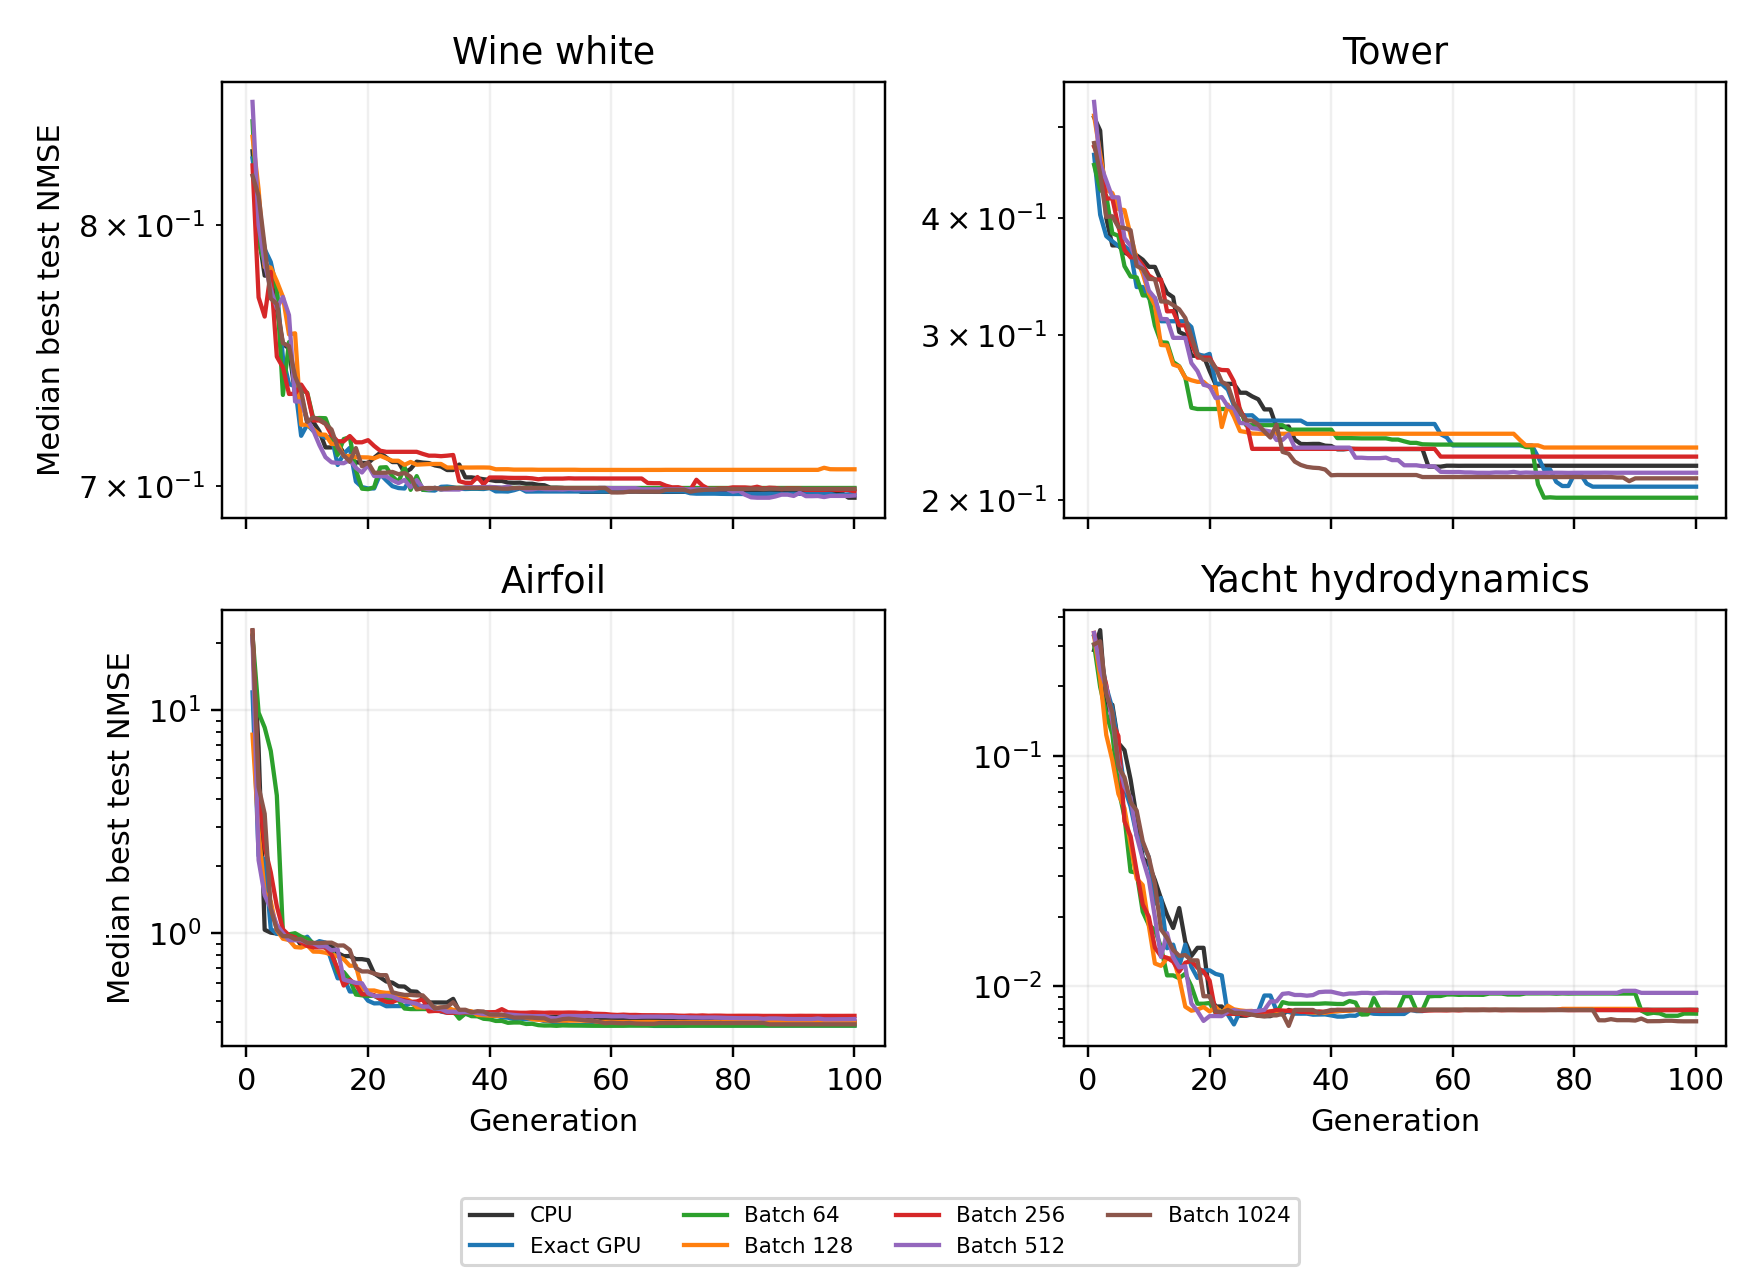
\includegraphics[height=0.72\textheight]{fitness_evolution}\\
  \footnotesize Batch size shifts the trajectory, not just runtime.
\end{frame}

\begin{frame}{RQ4 — Two regimes}
  \begin{columns}[T]
    \begin{column}{0.5\textwidth}
      \textbf{Exact path}
      \begin{itemize}\small
        \item Launch / sync bound (tiny programs).
        \item CUDA Graphs + pinned + fp32 target this.
        \item $\sim$1 program per graph launch.
      \end{itemize}
    \end{column}
    \begin{column}{0.5\textwidth}
      \textbf{Batched path}
      \begin{itemize}\small
        \item Occupancy bound, not launch bound.
        \item Hundreds of programs per launch.
        \item Gains from caches + sample-level occupancy.
      \end{itemize}
    \end{column}
  \end{columns}
  \vfill
  \centering
  \begin{block}{Cumulative optimization ablation (vs commit \texttt{851b0e9})}
    \centering exact \textbf{1.27$\times$} \qquad batch \textbf{1.72$\times$} wall-time
  \end{block}
\end{frame}

%==================================================================
\section{Conclusion}

\begin{frame}{Conclusion}
  \begin{itemize}
    \item GPU acceleration of GP fitness is \textbf{not} a single yes/no property.
    \item \exactgpu: useful when candidates carry enough sample work; preserves GOM decisions.
    \item \batchgpu: larger speedups via program-level parallelism, but \textbf{distorts search}.
    \item Acceleration must be reported \textbf{together with} search distortion.
  \end{itemize}
  \vfill
  \begin{exampleblock}{Future work}
    \small Full reference-paper matrix \,$\cdot$\, adaptive batch sizing \,$\cdot$\, mixed-precision acceptance checks.
  \end{exampleblock}
\end{frame}

\begin{frame}[plain]
  \centering
  \vfill
  {\Large Thank you}\\[1em]
  {\normalsize Questions?}
  \vfill
\end{frame}

\end{document}
